\documentclass[a4paper, 12pt]{article}
\usepackage[T2A]{fontenc}
\usepackage[utf8]{inputenc}
\usepackage[english,russian]{babel}
\usepackage{pgfplotstable}
\usepackage[normalem]{ulem}
\usepackage{geometry}
\usepackage{amsmath}
\usepackage{titlesec}
\usepackage{minted}

\pgfplotsset{compat=1.16}
\geometry{left=10mm, right=10mm, top=10mm, bottom=20mm}

\begin{document}
    \thispagestyle{empty}

\begin{center}
    Санкт-Петербургский политехнический университет Петра Великого\\
    Институт Компьютерных Наук и Технологий\\
    \bfseries{Кафедра «Высшая школа программной инженерии»}
\end{center}

\vspace{20ex}

\begin{center}
{
\LARGE \textbf{Курсовой проект} \\[3ex]
по дисциплине: «Микропроцессорные системы»
}
\end{center}

\vspace{40ex}

\noindent Выполнил\\
студент гр.33534/21\hfill
\begin{minipage}{0.7\textwidth}
    \hfill \uline{\hspace{3cm}} \hspace{1.1cm} С.А. Фомин
\end{minipage}

\vspace{3ex}

\noindent Проверил\\
преподаватель\hfill
\begin{minipage}{0.7\textwidth}
    \hfill \uline{\hspace{3cm}} \hspace{0.5cm} С.К. Круглов
\end{minipage}

\vspace{3ex}

\vfill

\begin{center}
    Санкт-Петербург\\
    2018
\end{center}



    \newpage

    \section*{Постановка задачи}
    Разработать клиент-серверное приложение для вывода на внешний жидкокристаллический
    дисплей (с помощью Raspberry Pi) количества сокращенных ссылок из базы данных сервиса short.taxnuke.ru в режиме реального времени.

    \section*{Ход работы}
    \begin{figure}
        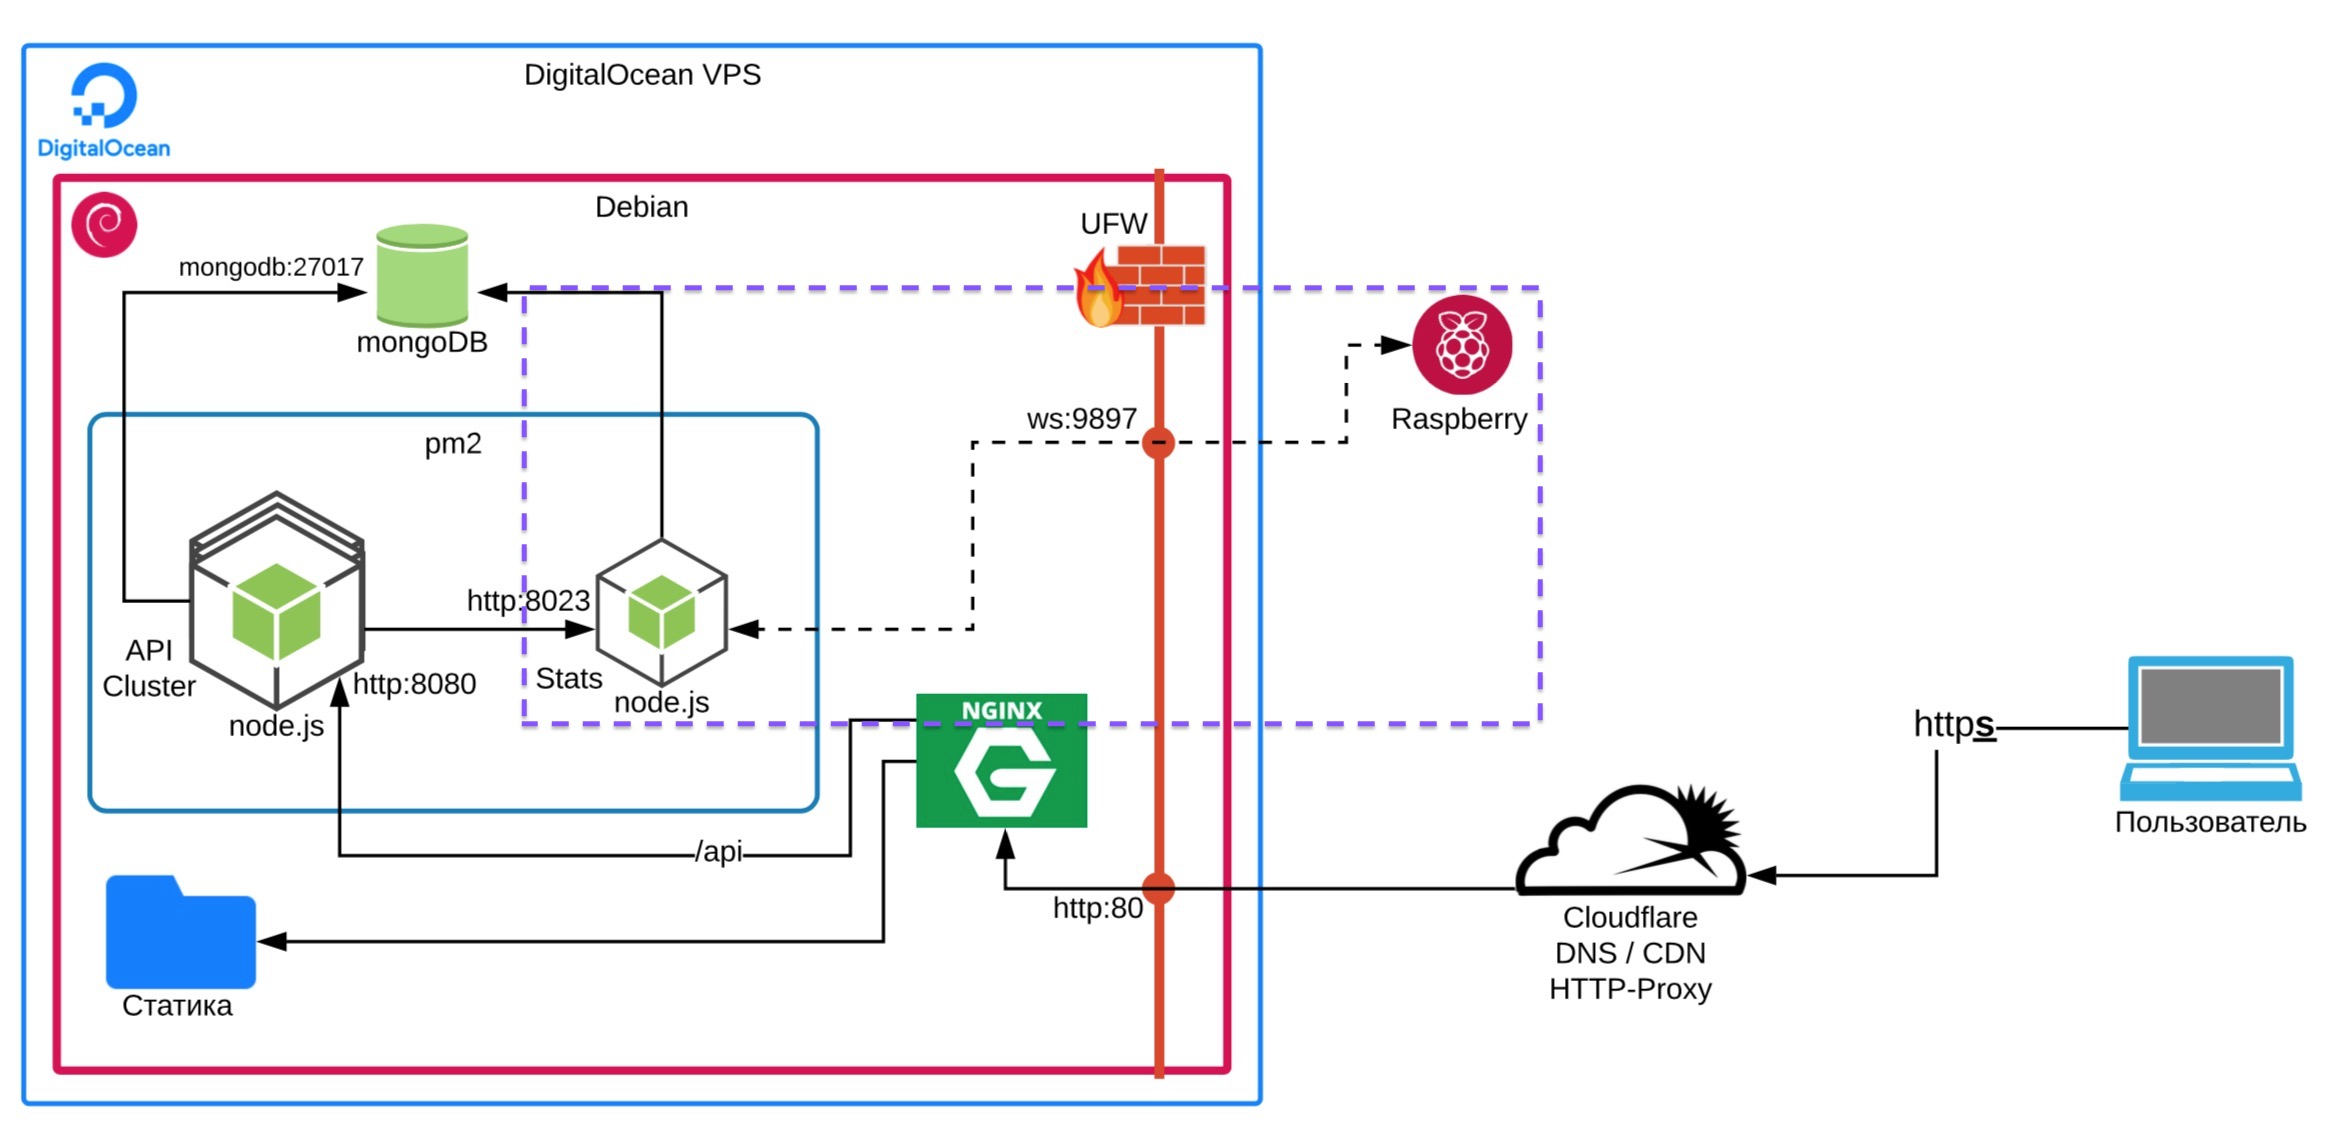
\includegraphics[width=\linewidth]{img/arch.jpg}
        \caption{Схема архитектуры крупным планом.}
        \label{fig:big_arch}
    \end{figure}

    На рисунке~\ref{fig:big_arch} изображена схема сервиса short.taxnuke.ru в целом, а также интегрированного в него
    разрабатываемого клиент-серверного приложения (в пунктирной фиолетовой рамке).

    В качестве программной среды было принятно решение использовать Node.js - кроссплатформенное решение,
    использующее в качестве JavaScript-движка V8, написанный на C. Для Node.js имеется множество готовых библиотек
    на JavaScript с привязками к нативным модулям на C++ и C и с многопоточностью.
    Выбор обусловлен тем, что изначально сервис short.taxnuke.ru тоже написан Node.js и использоание
    одной программной среды и языка позволяет минимизировать количество зависимостей и упростить интерфейс между компонентами.
    Также Node.js позволяет порождать дочерние процессы и передавать в них аргументы командной
    строки, управляющие последовательности и использовать потоки ввода/вывода.

    \subsection*{Проработка архитектуры и регламента взаимодействия между сервисами}
    В первую очередь необходимо было продумать, какие механизмы и средства будут использоваться для взаимодействия
    сервисом между собой и сервиса статистики и его потребителей. В качестве протокола для общения сервиса статистики и его клиентов
    было решено использовать websocket, чтобы избежать опрашивания основного
    сервиса (даже "длинного" опрашивания), которое неизбежно повлекло бы за собой ухудшение производительности основного сервиса
    при количестве клиентов (потребителей статистики оного), стремящемся к бесконечности.

    В качестве механизма взаимодействия сервисов между собой был выбран webhook, то есть один сервис будет
    отправлять http-запрос любым методом в любой эндпоинт другого сервиса с целью просто "дернуть" его и уведомить
    о том, что данные обновились. Было решено также не передавать с webhook никаких данных от одного сервиса к другому,
    это позволило избежать лишних развертываний основного сервиса по причинам изменений в интерфейсе сервиса статистики или формата данных.

    Вместо этого, сервис статистики открывает свое личное соединение с базой данных и по пришествии webhook сам
    параллельно отправляет к базе запрос и реализует там своими средствами всю бизнес логику, инкапсулируя ее от основного сервиса.

    \subsection*{Создание фундамента}
    Было принято решение использовать монорепозиторий git для управления контролем версий проекта, ввиду того, что
    логически это один т.н. микросервис, в дополнение к тому, что клиент и сервер изоморфны и используют одни библиотеки
    и написаны на одном языке.

    В качестве линтера (утилиты контроля стиля кода) используется eslint, его конфигурационный файл можно увидеть в
    %    todo: надо автоматически нумеровать
    приложении 4.

    В качестве системы доставки и развертки (деплоя) используется стандартная для Node.js связка из pm2 и git. pm2 на машине-разработчике
    подключается к машине-исполнителю по ssh, выполняет git clone, разворачивает проект из исходого кода и переставляет символьную ссылку
    на последний релиз, а так же берет на себя управление переменными окружения. Конфигурационный файл pm2 можно увидеть
    в приложении 3, он декларативен и не вызывает затруднений для понимания.

    \subsection*{Разработка сервиса-сервера}
    В качестве библиотеки для работы с websocket была выбрана самая популярная - "ws". Драйвер для общения с базой
    данных MongoDB было решено использовать официальный - "mongodb".

    При первом старте, сервер пытается подключиться к базе данных, если все произошло успешно, то создается http-сервер,
    который слушает на порт из переменной окружения, и аналогично далее создается websocket-сервер.

    При установлении нового соединения, сервер websocket отпрвляет тестовые данные для подтверждения соединения,
    и через 3 секунды отправляет клиенту актуальную информацию о статистике. Далее, websocket-сервер оповещает
    своих клиентов только после получения webhook от основного сервиса, при этом обновляя информацию о статистике.

    Исходный код сервера со множеством комментариев находится в приложении 1.

    \subsection*{Разработка сервиса-клиента}
    В качестве библиотеки для работы с websocket была также выбрана "ws". При старте, сервис-клиент пытается установить
    соединение с сервисом-сервером по протоколу websocket и далее выводит информацию на жидкокристаллический экран с помощью библиотеки
    "lcdi2c", которая позволяет абстрагироваться от низкоуровневой логики общения по протоколу I2C.
    Данную бибиотеку представляется возможным использовать благодаря её поддержки расширителя портов PCF8574, который был
    преобретен вместе с самим жидкокристаллическим экраном (16х2) на Hitachi HD44780 контроллере.
    Все библиотеки (пакеты) для Node.js можно найти на ресурсе npmjs.com, далее они подключаются как модули через функцию require.

    Исходный код клиента со множеством комментариев находится в приложении 2.

    \subsection*{Деплой (развертка) проекта на конечных устройствах}
    При внесении каких-либо изменений в проект, для их вступления в силу на реальных устройствах-носителях, необходимо
    выполнить процедуру деплоя, или "развертки". В качестве деплоера используется pm2, также обеспечивающий кластерный режим
    работы приложения и демонизацию (daemon режим работы).

    В первую очередь необходимо создать новый коммит с изменениями и выполнить пуш в удаленный репозиторий. Важно, чтобы
    конечные устройства имели свои SSH-ключи, которые добавлены в список доверенных для работы с удаленным репозиторием.
    После того, как эти шаги выполнены, сценарий деплоя различается в зависимости от того, деплой чего нужно произвести,
    клиентского сервиса или серверного.

    \subsubsection*{VPS-сервер DigitalOcean}
    В случае, если нужно задеплоить серверный сервис, из директории проекта нужно дать команду npm run deploy:server, или
    pm2 deploy vps, одна является псевдонимом другой.
    В результате выполнения этой команды, pm2 считает конфигурационный файл ecosystem.config.js, по содержимому которого
    будет определено, под каким пользователем нужно подключиться на VPS-сервер, из какого репозитория и куда сделать
    клонирование, и что сделать для самой развертки. Так же будут автоматически выставлены переменные окружения и выполнен
    бесшовный перезапуск приложения.

    Пример деплоя на сервер со снимками экрана приведен на рисунке~\ref{fig:deploy}.

    \begin{figure}
        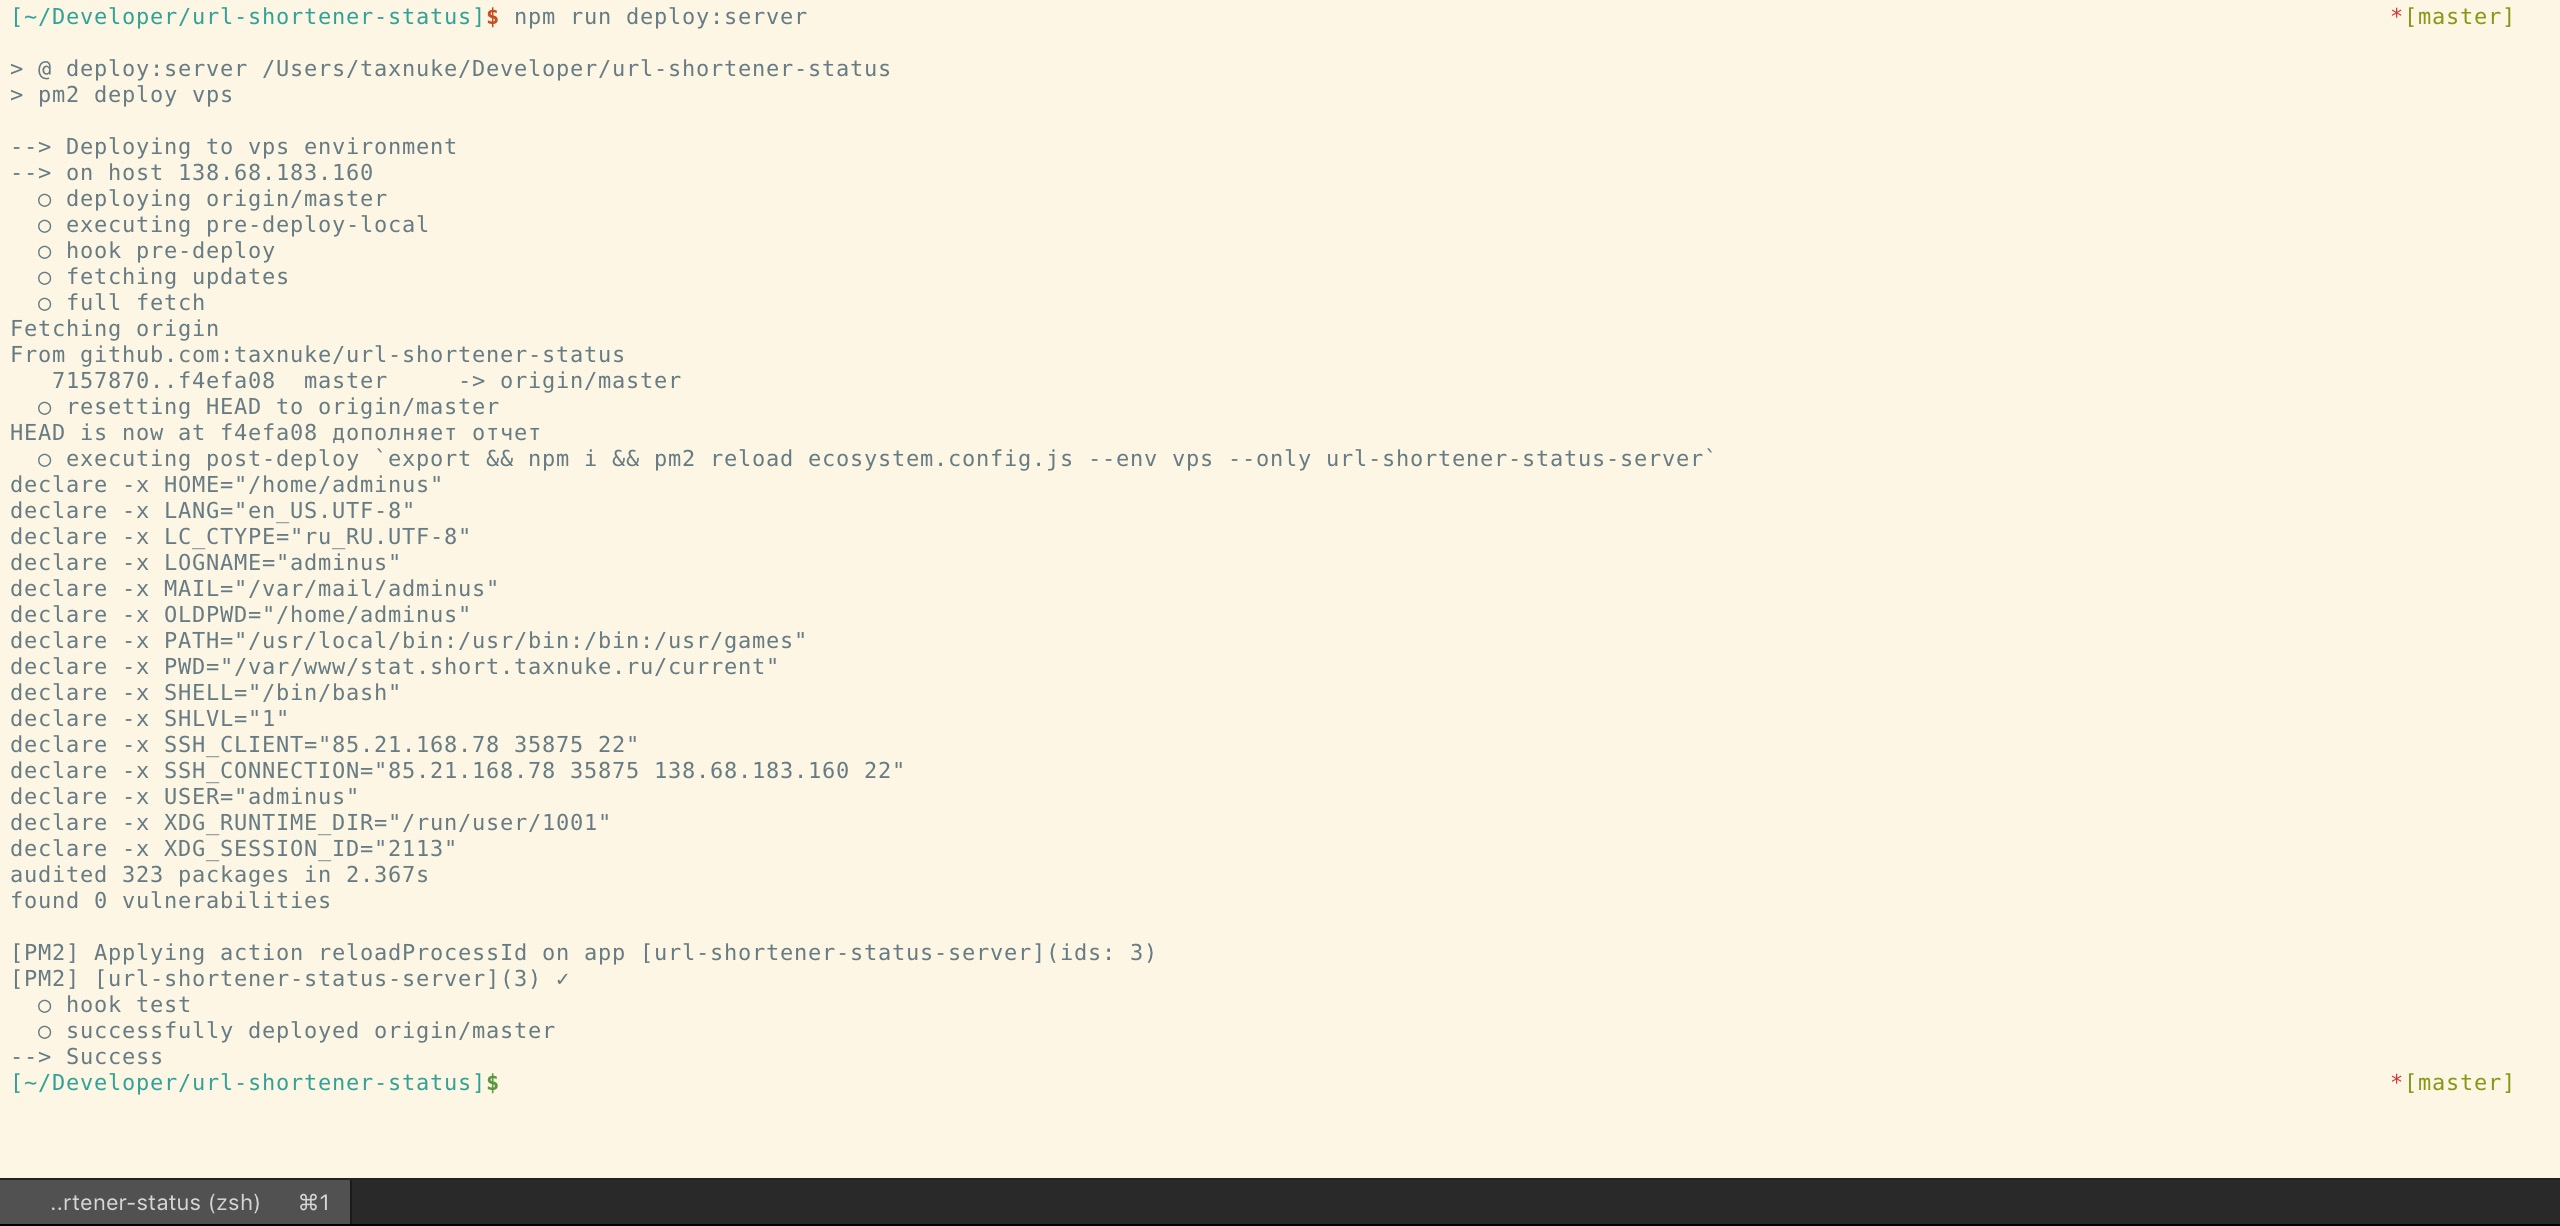
\includegraphics[width=\linewidth]{img/deploy.jpg}
        \caption{Ввод команды для деплоя и результат.}
        \label{fig:deploy}
    \end{figure}

    \subsubsection*{Raspberry Pi}
    В случае, если нужно задеплоить клиентский сервис, то из директории проекта нужно дать команду npm run deploy:client, или
    pm2 deploy raspberry, одна является псевдонимом другой. Далее будут выполнены те же действия, что и в результате
    деплоя на VPS, с тем лишь различием, что деплой на Raspberry в данном случае возможен лишь из локальной сети, так
    как ip в конфигурационном файле указан локальный, это сделано из соображений безопасности. Доступ к websocket-порту
    возможен также только с ip моего домашнего NAT, это контролируется фаерволом UFW.

    \section*{Результат работы}
    В результате выполнения курсового проекта было разработано серверное и клиентское приложения,
    работающие в паре и выполняющие поставленную задачу.

    \newpage
    \subsection*{ПРИЛОЖЕНИЕ 1. Код сервера}
    \inputminted{JavaScript}{../source/server.js}

    \newpage
    \subsection*{ПРИЛОЖЕНИЕ 2. Код клиента}
    \inputminted{JavaScript}{../source/client.js}

    \newpage
    \subsection*{ПРИЛОЖЕНИЕ 3. Содержимое конфигурационного файла для развертки}
    \inputminted{JavaScript}{../ecosystem.config.js}

    \newpage
    \subsection*{ПРИЛОЖЕНИЕ 4. Конфигурация линтера}
    \inputminted{JavaScript}{../.eslintrc.js}
\end{document}
